\documentclass[ProjectPlan_innit.tex]{subfiles}

\begin{document}

We plan to structure our project around four stages, namely Collection, Analysis, Writing and Review. 

\subsection{Collection}
In the collection phase we will outline what we want to know as basis for creating the survey. The survey will provide research foundation from numerous employees at Ericsson. Alongside the survey we will conduct interviews with additional employees. 

\subsection{Analysis}
The results of the surveys and interviews will serve as analysis material from which we can triangulate key areas of our report.

\subsection{Writing}
We outline the report to establish a foundation and then divide the sections to the members of the group. Each member writes his section, but we share research material on a common Git repository. The mother document will be a LaTeX document with modular documents, meaning that each member can write his section and later on link it to the mother documents that is already defined with a consistent formatting and style.

\subsection{Review}
We bring our individual parts together and review it as a single document, making sure it is consistent in language and expression. All parts will be revised as a result of feedback and criticism, and then bring it for final review with our main contact at Ericsson, Jesper Derehag.  

\smallskip

Figure 1 on page 4 shows a Gantt chart which represents our project schedule. 

\begin{figure*}[H!]
	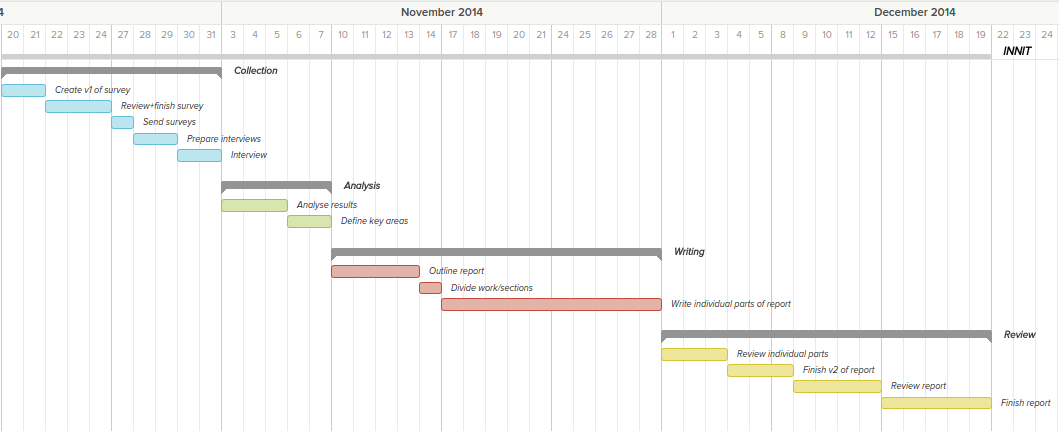
\includegraphics[width=\textwidth]{gantt.png}
	\caption{Figure 1 - Gantt chart visualising the project schedule.}
	\label{AAA}
\end{figure*}


\end{document}